% Search for all the places that say "PUT SOMETHING HERE".

\documentclass[11pt]{article}
\usepackage{amsmath,textcomp,amssymb,geometry,graphicx}

\def\Name{Jianzhong Chen}  % Your name
\def\Login{ee122-bv} % Your login
\def\Homework{1}%Number of Homework, PUT SOMETHING HERE
\def\Session{Fall 2013}


\title{EE122--Fall 2013 --- Solutions to Homework \Homework}
\author{\Name, \texttt{\Login}}
\markboth{CS170--\Session\  Homework \Homework\ \Name}{CS170--\Session\ Homework \Homework\ \Name, \texttt{\Login}}
\pagestyle{myheadings}

\begin{document}
\maketitle

\section*{Problem 1}
\label{pg:end-of-p1}


%Insert solution here

\subsection*{(1)}
$\dfrac{600*10^3}{3*10^8}+\dfrac{1200*8}{4*10^6}=4.4$ms
\subsection*{(2)}
\subsubsection*{(a)}
$\dfrac{600*10^3}{3*10^8}+\dfrac{10*10^6}{1000}*\dfrac{(1000+60)*8}{4*10^6}=21202$ms
\subsubsection*{(b)}
$\dfrac{10*8*10^6}{\dfrac{600*10^3}{3*10^8}+\dfrac{10*8*10^6}{1000}*\dfrac{1000+600}{4*10^6}}\approx{3.77*10^3}$bits/ms
\subsection*{(3)}
$\dfrac{1000*8}{4*10^6}+\dfrac{600*10^3}{3*10^8}+250*10^{-9}+\dfrac{80*8}{4*10^6}+\dfrac{600*10^3}{3*10^8}=6.41$ms
\subsection*{(4)}
$(\dfrac{1000*8}{4*10^6}+\dfrac{600*10^3}{3*10^8}+\dfrac{80*8}{4*10^6}+\dfrac{600*10^3}{3*10^8})*\dfrac{10*10^3}{1000}=61.6$ms


% Make sure that the solution here does not exceed one page here. If
% it does, use the extra space for this problem at the end.  
%
% Comment out the next line if you are NOT using the extra space
%\paragraph{} \emph{Continued on Page \pageref{pg:p1-continuation}}
\newpage


%%Do NOT remove/comment the next line
\pagestyle{plain}
%%It makes sure your name appears only on the first page
\section*{Problem 2}
$\dfrac{1500*8}{10^6}=0.012$s\\
$\dfrac{1500*8}{500*10^3}=0.024$s\\
$\dfrac{1500*8}{10^6}=0.012$s\\
$\dfrac{1500*8}{2*10^6}=0.006$s\\
$\dfrac{1500*8}{10^6}+2*10^{-3}=0.014$s\\
$\dfrac{1500*8}{500*10^{3}}+20*10^{-3}=0.044$s\\
$\dfrac{1500*8}{10^6}+30*10^{-3}=0.042$s\\
$\dfrac{1500*8}{2*10^6}+2*10^{-3}=0.008$s
\subsection*{Part (1)}
$0.014+0.044+0.042+0.008=0.108$s$=108$ms
\subsection*{Part (2)}
$0.014+20*10^{-3}+3*0.024+0.042+0.008=0.156$s$=156$ms
\subsection*{Part(3)}
\subsubsection*{(a)}
5 packets are dropped and 15packets reach Bob.
\subsubsection*{(b)}
Packet 11, Packet 13,Packet 15, Packet 17, Packet 19 are dropped.
\subsection*{(4)}
Because $\dfrac{0.00075}{0.0015}=1/2$ and $\dfrac{0.0015}{0.003}=1/2$\\
The fraction of his packets are lost is:\\
$\dfrac{1}{2}+\dfrac{1}{2}\times\dfrac{1}{2}=\dfrac{3}{4}$
\subsection*{(5)}
\subsubsection*{(a)}
$0.014+20*10^{-3}+5.5*0.024+0.042+0.008=0.216$s$=216$ms
\subsubsection*{(b)}
$0.008+30*10^{-3}+5.5*0.012+20*10^{-3}+5.5*0.024+0.014=0.27$s$=270$ms
\label{pg:end-of-p2}

%Insert solution here

% Make sure that the solution here does not exceed one page here. If
% it does, use the extra space for this problem at the end.  
%
% Comment out the next line if you are NOT using the extra space
%\paragraph{} \emph{Continued on Page \pageref{pg:p2-continuation}}



\newpage

\section*{Problem 3}

\subsection*{(1)}
$Z*2*10^{-3}+\dfrac{D}{B}*(Z-1)+\dfrac{D*M}{B*P}$
\subsection*{(2)}
$Z*2*10^{-3}+\dfrac{h}{B}*(Z-1)+\dfrac{D*M}{B*P}$
\subsection*{(3)}
$Z*2*10^{-3}+Z*\dfrac{k}{B}+Z*2*10^{-3}+\dfrac{k}{B}+Z*2*10^{-3}+\dfrac{M}{B}$
\subsection*{(4)}
\subsubsection*{(a)}
$T_{S\&F}=8*2*10^{-3}+\dfrac{1550*8}{50*10^6}*(8-1)+\dfrac{1550*8*3000*8}{50*10^6*(1550*8-50*8)}=0.018232$s$=18.232$ms\\
$T_{CTR}=8*2*10^{-3}+\dfrac{50*8}{59*10^6}*(8-1)+\dfrac{1550*8*3000*8}{50*10^6*(1550*8-50*8)}=0.016543$s$=16.543$ms\\
$T_{CS}=8*2*10^{-3}+8*\dfrac{100*8}{50*10^6}+8*2*10^{-3}+\dfrac{100*8}{50*10^6}+8*2*10^{-3}+\dfrac{3000*8}{50*10^6}=0.0486$s$=48.6$ms\\
So "Cut through routing" will transmit a 3000 byte file fastest.
\subsubsection*{(b)}
$T_{S\&F}=8*2*10^{-3}+\dfrac{1550*8}{50*10^6}*(8-1)+\dfrac{1550*8*30*8*10^6}{50*10^6*(1550*8-50*8)}=4.978$s\\
$T_{CTR}=8*2*10^{-3}+\dfrac{50*8}{59*10^6}*(8-1)+\dfrac{1550*8*30*8*10^6}{50*10^6*(1550*8-50*8)}=4.976$s\\
$T_{CS}=8*2*10^{-3}+8*\dfrac{100*8}{50*10^6}+8*2*10^{-3}+\dfrac{100*8}{50*10^6}+8*2*10^{-3}+\dfrac{30*8*10^6}{50*10^6}=4.848$s\\
So "circuit switching" will transmit a 30MB file fastest.
\label{pg:end-of-p3}

% Make sure that the solution here does not exceed one page here. If
% it does, use the extra space for this problem at the end.  
%
% Comment out the next line if you are NOT using the extra space
%\paragraph{} \emph{Continued on Page \pageref{pg:p3-continuation}}




\newpage

\section*{Problem 4}

\subsection*{(1)}
cmu.edu (Pittsburgh, PA)ping=79ms, dis=3626km, T=12.087ms\\
cs.brown.edu (Providence, RI)ping=93ms, dis=4303km, T=14.34ms\\
washington.edu (Seattle, WA)ping=23ms, dis=1082km, T=3.61ms\\
ucsd.edu (San Diego, CA)ping=14ms, dis=736km, T=2.45ms\\
uchicago.edu (Chicago, IL)ping=72ms, dis=2968km, T=9.89ms\\
columbia.edu (New York, NY)ping=87ms, dis=4117km, T=13.72ms\\
odu.edu (Norfolk, VA)ping=89ms, dis=4032km, T=13.44ms\\
stanford.edu (Palo Alto, CA)ping=4ms, dis=49km, T=0.16ms\\
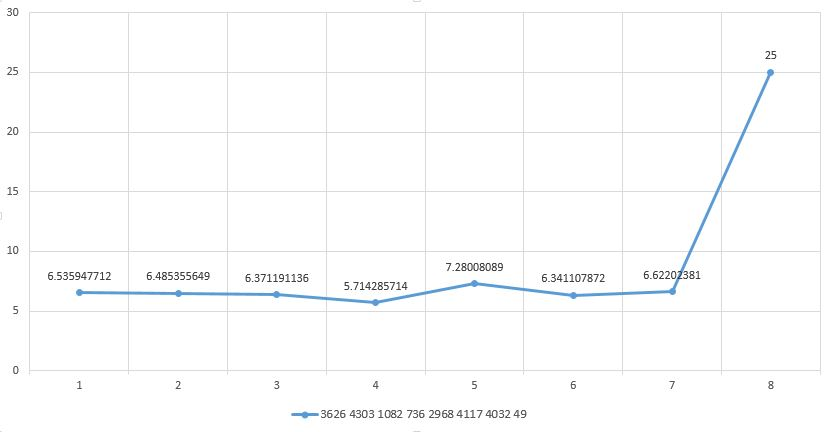
\includegraphics[scale=0.5]{Capture.JPG}
\subsection*{(2)}
Because there are transmitting delay, queuing delay, router processing time. The distance of transmission is actually larger than  the direct distance that we got from the website. Also the transmitting speed can not reach the speed of light.
\label{pg:end-of-p4}

% Make sure that the solution here does not exceed one page here. If
% it does, use the extra space for this problem at the end.  
%
% Comment out the next line if you are NOT using the extra space
%\paragraph{} \emph{Continued on Page \pageref{pg:p4-continuation}}


\newpage

%\section*{Problem 5}
%\label{pg:end-of-p5}

%Insert solution here


% Make sure that the solution here does not exceed one page here. If
% it does, use the extra space for this problem at the end.  
%
% Comment out the next line if you are NOT using the extra space
%\paragraph{} \emph{Continued on Page \pageref{pg:p5-continuation}}


%\newpage


%\section*{Problem 6}

%\subsection*{Part (a)}
%\subsection*{Part (b)}

%\label{pg:end-of-p6}

% Make sure that the solution here does not exceed one page here. If
% it does, use the extra space for this problem at the end.  
%
% Comment out the next line if you are NOT using the extra space
%\paragraph{} \emph{Continued on Page \pageref{pg:p6-continuation}}


%\newpage


%% Comment out the "extra spaces" completely for the problems for you
%% don't need them

%\section*{Extra space for Problem 1}
%\emph{Continued from Page \pageref{pg:end-of-p1}}\\

%Insert solution here


%\label{pg:p1-continuation}
%\newpage
%%Comment out the above three lines if you are not using extra space
%%for this problem.


%\section*{Extra space for Problem 2}
%\emph{Continued from Page \pageref{pg:end-of-p2}}\\

%Insert solution here

%\label{pg:p2-continuation}
%\newpage
%%Comment out the above three lines if you are not using extra space
%%for this problem.


%\section*{Extra space for Problem 3}
%\emph{Continued from Page \pageref{pg:end-of-p3}}\\

%Insert solution here

%\label{pg:p3-continuation}
%\newpage
%%Comment out the above three lines if you are not using extra space
%%for this problem.



%\section*{Extra space for Problem 4}
%\emph{Continued from Page \pageref{pg:end-of-p4}}\\

%Insert solution here

%\label{pg:p4-continuation}
%\newpage
%%Comment out the above three lines if you are not using extra space
%%for this problem.



%\section*{Extra space for Problem 5}
%\emph{Continued from Page \pageref{pg:end-of-p5}}\\

%Insert solution here


%\label{pg:p5-continuation}
%\newpage
%%Comment out the above three lines if you are not using extra space
%%for this problem.


%\section*{Extra space for Problem 6}
%\emph{Continued from Page \pageref{pg:end-of-p6}}\\


%Insert solution here


%\label{pg:p6-continuation}
%\newpage
%%Comment out the above three lines if you are not using extra space
%%for this problem.



\end{document}